\documentclass[aspectratio=169,12pt,t]{beamer}

% --- Theme: Metropolis (modern, clean) ---
\usetheme[progressbar=frametitle,numbering=fraction,block=fill]{metropolis}

% --- Fira Sans font (install texlive-fonts-extra if missing) ---
\IfFileExists{FiraSans.sty}{\usepackage[sfdefault]{FiraSans}}{}

% --- Light background with warm accent ---
\definecolor{mDarkTeal}{RGB}{35,55,59}
\definecolor{mLightBrown}{RGB}{235,228,216}
\definecolor{mAccent}{RGB}{140,70,20}

\setbeamercolor{normal text}{fg=mDarkTeal,bg=white}
\setbeamercolor{alerted text}{fg=mAccent}
\setbeamercolor{frametitle}{bg=mDarkTeal,fg=white}
\setbeamercolor{progress bar}{fg=mAccent,bg=mLightBrown}
\setbeamercolor{title separator}{fg=mAccent}
\setbeamercolor{progress bar in head/foot}{fg=mAccent,bg=mLightBrown}
\setbeamercolor{progress bar in section page}{fg=mAccent,bg=mLightBrown}

% --- Packages ---
\usepackage[utf8]{inputenc}
\usepackage{amsmath,amssymb,amsthm}
\usepackage{mathrsfs}
\usepackage{tikz}
\usetikzlibrary{arrows.meta,positioning,calc,decorations.pathreplacing,shapes,patterns}
\usepackage{pgfplots}
\pgfplotsset{compat=1.18}

% --- TikZ diagram styles (shared across the series) ---
\tikzset{
  axisln/.style={-{Stealth[length=2.6mm]}, line width=0.8pt, gray!75},
  curveln/.style={line width=1.6pt, line cap=round, line join=round},
  projln/.style={dash pattern=on 2.6pt off 2pt, line width=0.7pt},
  guide/.style={-{Stealth[length=2.6mm,width=2.2mm]}, line width=1.1pt},
}
% point marker with a white halo: \dotpt{color}{(coord)}
\newcommand{\dotpt}[2]{%
  \fill[white] #2 circle (3.6pt);
  \fill[#1] #2 circle (2.4pt);
}

% --- Semi-transparent white highlight for text on top of background images ---
\usepackage[most]{tcolorbox}

% Inline highlight: \hl{short text}
\newtcbox{\hl}{%
  nobeforeafter, tcbox raise base,
  colback=white, opacityback=0.6,
  colframe=white, opacityframe=0,
  sharp corners, boxsep=2pt, left=3pt, right=3pt, top=2pt, bottom=2pt%
}

% Block highlight: \begin{hlbox} ... \end{hlbox}  (multi-line, paragraphs, itemize)
% Optional argument accepts any tcolorbox key, e.g. [width=0.6\linewidth]
\newtcolorbox{hlbox}[1][]{%
  enhanced, breakable,
  colback=white, opacityback=0.6,
  colframe=white, opacityframe=0,
  boxsep=3pt, left=6pt, right=6pt, top=4pt, bottom=4pt,
  sharp corners,
  {#1}%
}

% --- Custom colors for content types ---
\definecolor{defcolor}{RGB}{25,85,120}
\definecolor{thmcolor}{RGB}{140,35,35}
\definecolor{proofcolor}{RGB}{35,100,50}
\definecolor{excolor}{RGB}{140,75,10}
\definecolor{remcolor}{RGB}{90,90,90}

% --- Beamer blocks for mathematical content types (semi-transparent) ---
\tcbset{hlblockbase/.style={
  enhanced, breakable,
  coltitle=white, fonttitle=\bfseries,
  opacitybacktitle=0.8, opacityback=0.6,
  opacityframe=0,
  sharp corners,
  boxsep=1pt, left=5pt, right=5pt, top=2pt, bottom=2pt,
  toptitle=1pt, bottomtitle=1pt
}}

\newtcolorbox{defblock}[1]{hlblockbase, title={#1},
  colbacktitle=defcolor, colback=defcolor!15, colframe=defcolor}
\newtcolorbox{thmblock}[1]{hlblockbase, title={#1},
  colbacktitle=thmcolor, colback=thmcolor!15, colframe=thmcolor}
\newtcolorbox{proofblock}[1]{hlblockbase, title={#1},
  colbacktitle=proofcolor, colback=proofcolor!15, colframe=proofcolor}
\newtcolorbox{exblock}[1]{hlblockbase, title={#1},
  colbacktitle=excolor, colback=excolor!15, colframe=excolor}
\newtcolorbox{remblock}[1]{hlblockbase, title={#1},
  colbacktitle=remcolor, colback=remcolor!15, colframe=remcolor}

% --- Metadata ---
\title{Chapter 5: Differentiation}
\subtitle{Section: Mean Value Theorems}
\author{Based on Walter Rudin's \emph{Principles of Mathematical Analysis}}
\date{}

\begin{document}

{
\usebackgroundtemplate{%
  
\includegraphics[width=\paperwidth,height=\paperheight,keepaspectratio=false]{chapter_05_bg_00.png}%
}
\begin{frame}[plain]
  \titlepage

  \note{
    Welcome to Chapter 5, Section 2: Mean Value Theorems. In the previous
    section we defined the derivative of a real function and developed the
    basic machinery for computing it. In this episode we prove some of the
    most useful theorems in all of calculus: the result that the derivative
    vanishes at interior extrema, the generalized mean value theorem, the
    mean value theorem itself, and the connection between the sign of the
    derivative and monotonicity. These results are the basis of nearly every
    application of differentiation. Let's get started.
  }
\end{frame}
}

{
\usebackgroundtemplate{%
  
\includegraphics[width=\paperwidth,height=\paperheight,keepaspectratio=false]{chapter_05_bg_01.png}%
}
\begin{frame}[c]{Outline}
  \begin{center}
    \tableofcontents
  \end{center}

  \note{
    Here is our plan. We first motivate why we need theorems that connect
    the derivative to the global behavior of a function. Then we define
    local maxima and minima and prove that the derivative vanishes at an
    interior extremum. With that tool in hand, we prove the generalized
    mean value theorem and deduce the classical mean value theorem from it.
    Finally, we harvest the first major payoff: the sign of the derivative
    controls whether a function is increasing, constant, or decreasing.
    We close with a summary and a look ahead.
  }
\end{frame}

\section{Motivation}

% --- Build 1/3 ---
\begin{frame}{From Local to Global}
  \begin{hlbox}
  \begin{itemize}
    \item $f'(x)$ captures the \alert{local} behavior of $f$ near a single point $x$
  \end{itemize}
  \end{hlbox}

  \note{
    Let's set the stage. Everything we did in the previous section was
    local. The derivative of "f" at a point "x" is a limit of difference
    quotients taken in an arbitrarily small neighborhood of "x". So the
    derivative at one point tells us, by itself, only how the function
    behaves very close to that point.
  }
\end{frame}

% --- Build 2/3 ---
\begin{frame}{From Local to Global}
  \begin{hlbox}
  \begin{itemize}
    \item $f'(x)$ captures the \alert{local} behavior of $f$ near a single point $x$
    \item Question: if we know $f'$ at \emph{every} point of an interval, what can we say about $f$ \alert{globally}?
  \end{itemize}
  \end{hlbox}

  \note{
    Here is the natural question. Suppose we know something about the
    derivative at every point of an interval. Can we draw conclusions about
    the function on the whole interval? For instance, if the derivative is
    zero everywhere, must the function be constant? This sounds obvious,
    but it needs a proof, and the proof requires a genuinely new idea.
  }
\end{frame}

% --- Build 3/3 ---
\begin{frame}{From Local to Global}
  \begin{hlbox}
  \begin{itemize}
    \item $f'(x)$ captures the \alert{local} behavior of $f$ near a single point $x$
    \item Question: if we know $f'$ at \emph{every} point of an interval, what can we say about $f$ \alert{globally}?
    \item Answer: \alert{mean value theorems} --- the bridge from local to global
    \item This section: Theorems 5.8 (Fermat), 5.9 (generalized MVT), 5.10 (MVT), 5.11 (monotonicity)
  \end{itemize}
  \end{hlbox}

  \note{
    The bridge from local to global is the mean value theorem. As you can
    see on the slide, we will prove four results. Theorem 5.8, often called
    Fermat's theorem, says the derivative vanishes at an interior extremum.
    Theorem 5.9 is the generalized mean value theorem for a pair of
    functions. Theorem 5.10 is the classical mean value theorem. And
    Theorem 5.11 uses it to link the sign of the derivative to
    monotonicity. Let's begin with local extrema.
  }
\end{frame}
}

{
\usebackgroundtemplate{%
  
\includegraphics[width=\paperwidth,height=\paperheight,keepaspectratio=false]{chapter_05_bg_02.png}%
}
\section{Local Extrema and the Derivative}

% --- Build 1/2 ---
\begin{frame}{Definition 5.7: Local Maximum and Minimum}
  \begin{defblock}{Definition 5.7: Local Maximum}
    Let $f$ be a real function defined on a metric space $X$. We say that
    $f$ has a \alert{local maximum} at a point $p \in X$ if there exists
    $\delta > 0$ such that
    \[
      f(q) \leq f(p) \quad \text{for all } q \in X \text{ with } d(p, q) < \delta.
    \]
  \end{defblock}

  \vspace{0.3em}
  \hl{\emph{Local minima} are defined likewise (with $f(q) \geq f(p)$).}

  \note{
    We start with the key definition. A function "f" has a local maximum at
    a point "p" if there is some positive radius delta such that the value
    of "f" at "p" is at least as large as the value at every point "q"
    within distance delta of "p". Note two things. First, the definition is
    stated for a real valued function on an arbitrary metric space, not
    just on an interval. Second, the inequality is not strict, so a
    constant function has a local maximum at every point. Local minima are
    defined the same way with the inequality reversed.
  }
\end{frame}

% --- Build 2/2 ---
\begin{frame}{Definition 5.7: Local Maximum and Minimum}
  \begin{defblock}{Definition 5.7: Local Maximum}
    Let $f$ be a real function defined on a metric space $X$. We say that
    $f$ has a \alert{local maximum} at a point $p \in X$ if there exists
    $\delta > 0$ such that
    \[
      f(q) \leq f(p) \quad \text{for all } q \in X \text{ with } d(p, q) < \delta.
    \]
  \end{defblock}

  \begin{center}
  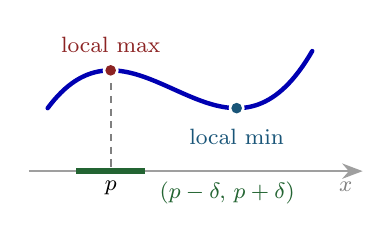
\begin{tikzpicture}[scale=0.8]
    % Axis
    \draw[axisln] (-0.3,0) -- (5.0,0) node[below left, gray]{\footnotesize $x$};
    % Curve: f(x) = 0.15x^3 - 0.9x^2 + 1.35x + 1
    %   f'(x) = 0.45(x-1)(x-3): local max at (1, 1.6), local min at (3, 1.0)
    \draw[curveln, blue!70!black, domain=0:4.2, samples=80]
      plot (\x, {0.15*\x^3 - 0.9*\x^2 + 1.35*\x + 1});
    % Local max at (1, 1.6)
    \draw[projln, gray] (1,1.6) -- (1,0);
    \dotpt{thmcolor}{(1,1.6)}
    \node[thmcolor, above=3pt] at (1,1.6) {\footnotesize local max};
    % Neighborhood (p - delta, p + delta) on the axis
    \draw[line width=2.2pt, proofcolor] (0.45,0) -- (1.55,0);
    \node[below, black] at (1,0) {\footnotesize $p$};
    \node[proofcolor, below] at (2.85,-0.02) {\footnotesize $(p-\delta,\, p+\delta)$};
    % Local min at (3, 1.0)
    \dotpt{defcolor}{(3,1.0)}
    \node[defcolor, below=4pt] at (3,1.0) {\footnotesize local min};
  \end{tikzpicture}
  \end{center}

  \note{
    The picture shows what the definition means on the real line. The blue
    curve is the graph of "f". The dark red point at the top of the first
    hill is a local maximum: on the green interval on the axis, from "p"
    minus delta to "p" plus delta, no value of "f" exceeds the value at
    "p". The blue point in the valley further right is a local minimum.
    Note that a local maximum need not be the largest value of the function
    overall; the curve climbs higher again at the far right. Next, we prove
    the fundamental fact about derivatives at such points.
  }
\end{frame}

% --- Build 1/2 ---
\begin{frame}{Theorem 5.8: The Derivative Vanishes at Interior Extrema}
  \begin{thmblock}{Theorem 5.8}
    Let $f$ be defined on $[a, b]$. If $f$ has a local maximum at a point
    $x \in (a, b)$, and if $f'(x)$ exists, then
    \[
      \boxed{f'(x) = 0.}
    \]
  \end{thmblock}

  \vspace{0.3em}
  \hl{The analogous statement for local \emph{minima} is also true.}

  \note{
    Here is Theorem 5.8, the basis of many applications of differentiation.
    It is often called Fermat's theorem. Suppose "f" is defined on the
    closed interval from "a" to "b", and suppose it has a local maximum at
    an interior point "x". If the derivative of "f" exists at that point,
    then it must be zero. The same conclusion holds at a local minimum.
    Both hypotheses matter: the point must lie strictly inside the
    interval, and the derivative must actually exist there. At an endpoint,
    or at a corner where the derivative fails to exist, the conclusion can
    fail. One more caution: the converse is false. The derivative of "x"
    cubed vanishes at zero, yet zero is not a local extremum; a zero
    derivative only marks a candidate. Let's see why the theorem is true.
  }
\end{frame}

% --- Build 2/2 ---
\begin{frame}[c]{Theorem 5.8: The Derivative Vanishes at Interior Extrema}
  \begin{center}
  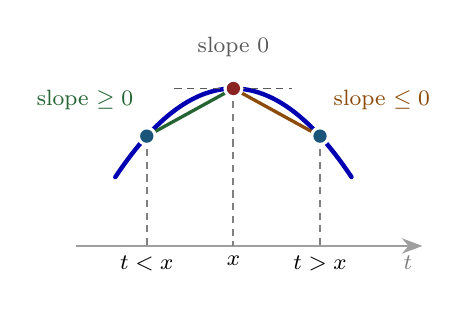
\begin{tikzpicture}[scale=1.0]
    % Axis
    \draw[axisln] (0,0) -- (4.4,0) node[below left, gray]{\footnotesize $t$};
    % Curve: cap with max at (2,2)
    \draw[curveln, blue!70!black, domain=0.5:3.5, samples=60]
      plot (\x, {2-0.5*(\x-2)^2});
    % Horizontal tangent at the max (the conclusion)
    \draw[projln, remcolor] (1.25,2) -- (2.75,2);
    \node[remcolor, above=8pt] at (2,2) {\footnotesize slope $0$};
    % Left secant
    \draw[proofcolor, line width=1.2pt] (0.9,1.395) -- (2,2);
    \node[proofcolor, anchor=east] at (0.85,1.85) {\footnotesize slope $\geq 0$};
    \draw[projln, gray] (0.9,1.395) -- (0.9,0) node[below, black]{\footnotesize $t < x$};
    \dotpt{defcolor}{(0.9,1.395)}
    % Right secant
    \draw[excolor, line width=1.2pt] (2,2) -- (3.1,1.395);
    \node[excolor, anchor=west] at (3.15,1.85) {\footnotesize slope $\leq 0$};
    \draw[projln, gray] (3.1,1.395) -- (3.1,0) node[below, black]{\footnotesize $t > x$};
    \dotpt{defcolor}{(3.1,1.395)}
    % Max point
    \draw[projln, gray] (2,2) -- (2,0) node[below, black]{\footnotesize $x$};
    \dotpt{thmcolor}{(2,2)}
  \end{tikzpicture}
  \end{center}

  \hl{\textbf{Key idea:} compare the \alert{one-sided} difference quotients at the maximum.}

  \note{
    The picture reveals the whole proof. The red point at the top is the
    local maximum at "x". Take a nearby point "t" to the left of "x": the
    green chord from that point up to the maximum rises from left to right,
    so its slope is greater than or equal to zero. Now take a point "t" to
    the right: the orange chord falls, so its slope is at most zero. As "t"
    approaches "x", both chord slopes converge to the same number, the
    derivative at "x". A number that is both at least zero and at most zero
    must be zero; the dashed horizontal segment through the peak shows this
    conclusion, a tangent of slope zero. Let's now write the argument out
    carefully.
  }
\end{frame}

% --- Build 1/4 ---
\begin{frame}{Proof of Theorem 5.8}
  \begin{proofblock}{Step 1: Set up the neighborhood}
    Choose $\delta$ as in Definition 5.7 so that
    $a < x - \delta < x < x + \delta < b$;
    on this neighborhood, $f(t) \leq f(x)$.
  \end{proofblock}

  \note{
    Step 1 is pure setup. Since "x" is a local maximum, Definition 5.7
    gives us a delta such that "f" of "t" is at most "f" of "x" for all "t"
    within delta of "x". Because "x" lies strictly between "a" and "b", we
    may shrink delta so the whole neighborhood stays inside the interval.
    This is exactly where we use the assumption that "x" is an interior
    point. Next, we look at difference quotients from the left.
  }
\end{frame}

% --- Build 2/4 ---
\begin{frame}{Proof of Theorem 5.8}
  \begin{proofblock}{Step 1: Set up the neighborhood}
    Choose $\delta$ as in Definition 5.7 so that
    $a < x - \delta < x < x + \delta < b$;
    on this neighborhood, $f(t) \leq f(x)$.
  \end{proofblock}

  \begin{proofblock}{Step 2: Approach from the left $\Rightarrow f'(x) \geq 0$}
    If $x - \delta < t < x$, then
    $\frac{f(t) - f(x)}{t - x} \geq 0$.
    Letting $t \to x$ gives $f'(x) \geq 0$.
  \end{proofblock}

  \note{
    Step 2: take "t" slightly to the left of "x". The numerator, "f" of "t"
    minus "f" of "x", is at most zero because "x" is a local maximum. The
    denominator, "t" minus "x", is negative. A nonpositive number divided
    by a negative number is nonnegative, so the difference quotient is at
    least zero. Since the derivative exists at "x", we can let "t" tend to
    "x" and the inequality survives the limit: the derivative is at least
    zero. Now we play the same game from the right.
  }
\end{frame}

% --- Build 3/4 ---
\begin{frame}{Proof of Theorem 5.8}
  \begin{proofblock}{Step 1: Set up the neighborhood}
    Choose $\delta$ as in Definition 5.7 so that
    $a < x - \delta < x < x + \delta < b$;
    on this neighborhood, $f(t) \leq f(x)$.
  \end{proofblock}

  \begin{proofblock}{Step 2: Approach from the left $\Rightarrow f'(x) \geq 0$}
    If $x - \delta < t < x$, then
    $\frac{f(t) - f(x)}{t - x} \geq 0$.
    Letting $t \to x$ gives $f'(x) \geq 0$.
  \end{proofblock}

  \begin{proofblock}{Step 3: Approach from the right $\Rightarrow f'(x) \leq 0$}
    If $x < t < x + \delta$, then
    $\frac{f(t) - f(x)}{t - x} \leq 0$,
    so $f'(x) \leq 0$.
  \end{proofblock}

  \note{
    Step 3 mirrors step 2. Take "t" slightly to the right of "x". The
    numerator is still at most zero, but now the denominator is positive,
    so the quotient is at most zero. Letting "t" tend to "x" from the right
    gives that the derivative is at most zero. We now have two inequalities
    pointing in opposite directions, and the conclusion is immediate.
  }
\end{frame}

% --- Build 4/4 ---
\begin{frame}{Proof of Theorem 5.8}
  \begin{proofblock}{Step 1: Set up the neighborhood}
    Choose $\delta$ as in Definition 5.7 so that
    $a < x - \delta < x < x + \delta < b$;
    on this neighborhood, $f(t) \leq f(x)$.
  \end{proofblock}

  \begin{proofblock}{Step 2: Approach from the left $\Rightarrow f'(x) \geq 0$}
    If $x - \delta < t < x$, then
    $\frac{f(t) - f(x)}{t - x} \geq 0$.
    Letting $t \to x$ gives $f'(x) \geq 0$.
  \end{proofblock}

  \begin{proofblock}{Step 3: Approach from the right $\Rightarrow f'(x) \leq 0$}
    If $x < t < x + \delta$, then
    $\frac{f(t) - f(x)}{t - x} \leq 0$,
    so $f'(x) \leq 0$.
  \end{proofblock}

  \vspace{-0.7em}
  \hl{Hence $\boxed{f'(x) = 0.}$ \quad $\blacksquare$}

  \note{
    Combining steps 2 and 3, the derivative at "x" is at least zero and at
    most zero, hence exactly zero. That completes the proof of Theorem 5.8.
    This little result is the engine behind everything that follows: it
    lets us convert the existence of an interior extremum into an equation
    about the derivative. With it we can now attack the mean value
    theorems themselves.
  }
\end{frame}
}

{
\usebackgroundtemplate{%
  
\includegraphics[width=\paperwidth,height=\paperheight,keepaspectratio=false]{chapter_05_bg_03.png}%
}
\section{The Mean Value Theorems}

\begin{frame}{Theorem 5.9: Generalized Mean Value Theorem}
  \begin{thmblock}{Theorem 5.9 (Generalized MVT)}
    If $f$ and $g$ are continuous real functions on $[a, b]$ which are
    differentiable in $(a, b)$, then there is a point $x \in (a, b)$ at which
    \[
      [f(b) - f(a)]\, g'(x) = [g(b) - g(a)]\, f'(x).
    \]
  \end{thmblock}

  \vspace{0.3em}
  \begin{hlbox}
  \begin{itemize}
    \item Differentiability is \alert{not} required at the endpoints $a$, $b$
    \item Also known as the \emph{Cauchy mean value theorem}
  \end{itemize}
  \end{hlbox}

  \note{
    Here is the first main result: the generalized mean value theorem, also
    named after Cauchy. It concerns two functions at once. Both "f" and "g"
    are continuous on the closed interval and differentiable on the open
    interval. The conclusion is that at some interior point "x", the
    increment of "f" over the whole interval times the derivative of "g" at
    "x" equals the increment of "g" times the derivative of "f" at "x".
    Notice from the first bullet that we need differentiability only at
    interior points; continuity at the endpoints suffices. This weaker
    hypothesis costs nothing in the proof and is often useful. Before the
    proof, let's plan our strategy.
  }
\end{frame}

\begin{frame}{Proof Strategy: Theorem 5.9}
  \begin{hlbox}
  \textbf{Goal:} Find $x \in (a,b)$ where a certain derivative vanishes.

  \vspace{0.3em}
  \textbf{Approach:}
  \begin{enumerate}
    \item Combine $f$ and $g$ into a single auxiliary function $h$
    \item Arrange $h(a) = h(b)$ --- the increments cancel by design
    \item $h$ attains a maximum and a minimum on $[a,b]$ (Theorem 4.16)
    \item If $h$ is not constant, some extremum is \emph{interior}; apply Theorem 5.8
  \end{enumerate}
  \end{hlbox}

  \begin{remblock}{Recall: Theorem 4.16}
    A continuous real function on a compact set attains its maximum and minimum.
  \end{remblock}

  \note{
    Let's understand the plan before diving in. The desired equation says
    that a certain combination of derivatives vanishes at "x". So we build
    one auxiliary function "h" whose derivative is exactly that
    combination. The function is designed so that its values at the two
    endpoints agree; the increments of "f" and "g" cancel each other. Then
    we bring in Theorem 4.16 from Chapter 4, shown in the gray box: a
    continuous function on a compact set, such as a closed bounded
    interval, attains a maximum and a minimum. If "h" is not constant, at
    least one of these extrema must occur strictly inside the interval,
    and Theorem 5.8 forces the derivative of "h" to vanish there. Now the
    details.
  }
\end{frame}

% --- Build 1/4 ---
\begin{frame}{Proof of Theorem 5.9}
  \begin{proofblock}{Step 1: The auxiliary function}
    Put
    \[
      h(t) = [f(b) - f(a)]\, g(t) - [g(b) - g(a)]\, f(t)
      \qquad (a \leq t \leq b).
    \]
    Then $h$ is continuous on $[a, b]$ and differentiable in $(a, b)$.
  \end{proofblock}

  \note{
    Step 1 defines the auxiliary function "h". It is a fixed linear
    combination of "g" and "f": the increment of "f" over the interval
    multiplies "g" of "t", and the increment of "g" multiplies "f" of "t",
    with a minus sign in between. The coefficients are constants, so "h"
    inherits continuity on the closed interval and differentiability on
    the open interval from "f" and "g". Note that the derivative of "h" at
    a point is exactly the expression we want to prove equal to zero. Next
    we check the endpoint values.
  }
\end{frame}

% --- Build 2/4 ---
\begin{frame}{Proof of Theorem 5.9}
  \begin{proofblock}{Step 1: The auxiliary function}
    Put
    \[
      h(t) = [f(b) - f(a)]\, g(t) - [g(b) - g(a)]\, f(t)
      \qquad (a \leq t \leq b).
    \]
    Then $h$ is continuous on $[a, b]$ and differentiable in $(a, b)$.
  \end{proofblock}

  \begin{proofblock}{Step 2: Equal endpoint values}
    \begin{equation}
      h(a) = f(b)g(a) - f(a)g(b) = h(b) \tag{12}
    \end{equation}
    It remains to show: $h'(x) = 0$ for some $x \in (a, b)$.
  \end{proofblock}

  \note{
    Step 2 is a small computation. Evaluate "h" at the left endpoint: the
    cross terms "f" of "b" times "g" of "a" and "f" of "a" times "g" of
    "b" survive, while the products of values at the same endpoint cancel.
    Evaluating at "b" gives exactly the same expression, which is equation
    12 on the slide. So "h" takes equal values at the two endpoints, just
    as the strategy demanded. Incidentally, a differentiable function with
    equal endpoint values is exactly the setting of Rolle's theorem; our
    auxiliary function was engineered to land in that special case. The
    theorem is now reduced to a single claim:
    the derivative of "h" vanishes somewhere strictly between "a" and "b".
    We prove this by considering three cases.
  }
\end{frame}

% --- Build 3/4 ---
\begin{frame}{Proof of Theorem 5.9}
  \begin{proofblock}{Step 2 (recap)}
    $h(a) = h(b)$ by (12); \quad goal: $h'(x) = 0$ for some $x \in (a, b)$.
  \end{proofblock}

  \begin{proofblock}{Step 3: Case analysis}
    \begin{itemize}
      \item If $h$ is \emph{constant}: $h'(x) = 0$ for every $x \in (a,b)$. \checkmark
      \item If $h(t) > h(a)$ for some $t \in (a, b)$: $h$ attains its
        \alert{maximum} at some $x$ (Theorem 4.16); by (12), $x \in (a, b)$,
        so Theorem 5.8 gives $h'(x) = 0$. \checkmark
    \end{itemize}
  \end{proofblock}

  \note{
    Step 3 splits into cases. If "h" is constant, its derivative vanishes
    everywhere, and we are done. Otherwise, suppose "h" climbs above its
    endpoint value somewhere inside the interval. By Theorem 4.16, "h"
    attains its maximum at some point "x" of the closed interval. The
    maximum value exceeds the common endpoint value, so by equation 12 the
    point "x" cannot be an endpoint; it must be interior. And now Theorem
    5.8 does its job: at an interior maximum where the derivative exists,
    the derivative is zero. One case remains.
  }
\end{frame}

% --- Build 4/4 ---
\begin{frame}{Proof of Theorem 5.9}
  \begin{proofblock}{Step 2 (recap)}
    $h(a) = h(b)$ by (12); \quad goal: $h'(x) = 0$ for some $x \in (a, b)$.
  \end{proofblock}

  \begin{proofblock}{Step 3: Case analysis}
    \begin{itemize}
      \item If $h$ is \emph{constant}: $h'(x) = 0$ for every $x \in (a,b)$. \checkmark
      \item If $h(t) > h(a)$ for some $t \in (a, b)$: $h$ attains its
        \alert{maximum} at some $x$ (Theorem 4.16); by (12), $x \in (a, b)$,
        so Theorem 5.8 gives $h'(x) = 0$. \checkmark
      \item If $h(t) < h(a)$ for some $t \in (a, b)$: same argument with the
        \alert{minimum} of $h$. \checkmark
    \end{itemize}
  \end{proofblock}

  \vspace{-0.7em}
  \hl{$h'(x) = 0$ unpacks to $\boxed{[f(b)-f(a)]\,g'(x) = [g(b)-g(a)]\,f'(x).}$ \quad $\blacksquare$}

  \note{
    In the last case, "h" dips below its endpoint value somewhere inside.
    Then we pick "x" where "h" attains its minimum; again equation 12
    forces "x" to be interior, and Theorem 5.8 gives a vanishing
    derivative. In every case we found an interior point where the
    derivative of "h" is zero. Unpacking the definition of "h", that
    equation is precisely the conclusion of the theorem, boxed at the
    bottom of the slide. Notice how little we assumed: no differentiability
    at the endpoints, and no assumption that "g" prime is nonzero. Next,
    the most famous special case.
  }
\end{frame}

% --- Build 1/2 ---
\begin{frame}{Theorem 5.10: The Mean Value Theorem}
  \begin{thmblock}{Theorem 5.10 (Mean Value Theorem)}
    If $f$ is a real continuous function on $[a, b]$ which is differentiable
    in $(a, b)$, then there is a point $x \in (a, b)$ at which
    \[
      f(b) - f(a) = (b - a)\, f'(x).
    \]
  \end{thmblock}

  \vspace{0.3em}
  \begin{hlbox}
  Some tangent line is \alert{parallel to the secant line} through the endpoints.
  \end{hlbox}
  
  \note{
    Here it is: the mean value theorem, the special case that gives the
    whole section its name. If "f" is continuous on the closed interval
    and differentiable inside, then at some interior point "x" the
    increment of "f" over the interval equals the length of the interval
    times the derivative at "x". Dividing by "b" minus "a", the statement
    says the average rate of change over the interval is achieved as an
    instantaneous rate of change somewhere inside. Think of driving: if
    your average speed over a trip was sixty miles per hour, then at some
    instant your speedometer read exactly sixty. In geometric language,
    written below the box: some tangent line to the graph is parallel to
    the secant line joining the two endpoints. A picture makes this
    vivid.
  }
\end{frame}

% --- Build 2/2 ---
\begin{frame}[c]{Theorem 5.10: The Mean Value Theorem}
  \begin{center}
  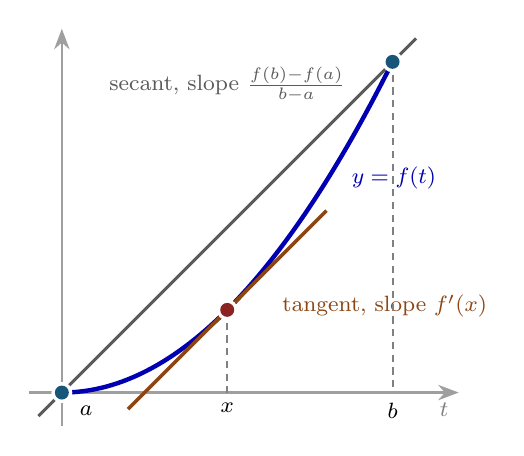
\begin{tikzpicture}[scale=1.05]
    % Axes
    \draw[axisln] (-0.4,0) -- (4.8,0) node[below left, gray]{\footnotesize $t$};
    \draw[axisln] (0,-0.4) -- (0,4.4);
    % Curve f(t) = t^2/4
    \draw[curveln, blue!70!black, domain=0:4, samples=60] plot (\x, {\x*\x/4});
    \node[blue!70!black, right, fill=white, inner sep=1.5pt]
      at (3.45,2.6) {\footnotesize $y = f(t)$};
    % Secant through the endpoints
    \draw[remcolor, line width=1.1pt, shorten <=-12pt, shorten >=-12pt]
      (0,0) -- (4,4);
    \node[remcolor, above left] at (3.55,3.4)
      {\footnotesize secant, slope $\frac{f(b)-f(a)}{b-a}$};
    % Tangent at x = 2: y = t - 1 (parallel to the secant)
    \draw[mAccent, line width=1.3pt] (0.8,-0.2) -- (3.2,2.2);
    \node[mAccent, below right] at (2.55,1.3)
      {\footnotesize tangent, slope $f'(x)$};
    % Endpoints and the mean value point
    \node[below right, black] at (0.1,-0.04) {\footnotesize $a$};
    \draw[projln, gray] (4,4) -- (4,0) node[below, black]{\footnotesize $b$};
    \draw[projln, gray] (2,1) -- (2,0) node[below, black]{\footnotesize $x$};
    \dotpt{defcolor}{(0,0)}
    \dotpt{defcolor}{(4,4)}
    \dotpt{thmcolor}{(2,1)}
  \end{tikzpicture}
  \end{center}

  \note{
    Let's read the picture. The blue curve is the graph of "f" on the
    interval from "a" to "b". The gray line is the secant through the two
    endpoint values, marked by blue dots; its slope is the increment of
    "f" divided by "b" minus "a", the average rate of change. The orange
    line is tangent to the curve at the interior point "x", marked in red,
    and it is parallel to the gray secant: its slope, the derivative at
    "x", equals the secant slope.
    The theorem promises that such a point "x" always exists, though it
    does not tell us where it is or whether it is unique. The proof is
    now a one-liner.
  }
\end{frame}

\begin{frame}{Proof of Theorem 5.10}
  \begin{proofblock}{Proof}
    Take $g(t) = t$ in Theorem 5.9. Then $g(b) - g(a) = b - a$ and
    $g'(x) = 1$, so
    \[
      [f(b) - f(a)] \cdot 1 = (b - a)\, f'(x). \qquad \blacksquare
    \]
  \end{proofblock}

  \vspace{0.5em}
  \begin{hlbox}
  \textbf{Technique:} prove the general two-function statement first;
  the classical result is the special case $g(t) = t$.
  \end{hlbox}

  \note{
    The proof is delightfully short. In the generalized mean value theorem,
    choose "g" to be the identity function. Its increment over the interval
    is "b" minus "a", and its derivative is one everywhere. Substituting
    these into the conclusion of Theorem 5.9 gives exactly the mean value
    theorem. This is a pattern worth remembering, highlighted at the bottom
    of the slide: sometimes the cleanest path to a classical result is
    through a more general statement whose symmetry makes the proof easier.
    Now let's collect the first major payoff of the mean value theorem.
  }
\end{frame}
}

{
\usebackgroundtemplate{%
  
\includegraphics[width=\paperwidth,height=\paperheight,keepaspectratio=false]{chapter_05_bg_04.png}%
}
\section{Monotonicity from the Sign of the Derivative}

% --- Build 1/3 ---
\begin{frame}{Theorem 5.11: The Sign of $f'$ Controls Monotonicity}
  \begin{thmblock}{Theorem 5.11}
    Suppose $f$ is differentiable in $(a, b)$.
    \begin{enumerate}
      \item[(a)] If $f'(x) \geq 0$ for all $x \in (a, b)$, then $f$ is
        \alert{monotonically increasing}.
    \end{enumerate}
  \end{thmblock}

  \note{
    Here is the payoff. Suppose "f" is differentiable on an open interval.
    Part "a" says that if the derivative is nonnegative at every point,
    then the function is monotonically increasing. Recall from Chapter 4
    that monotonically increasing means: whenever one point is less than
    another, the value of "f" at the first is less than or equal to the
    value at the second. This is the rigorous version of the intuition
    that a nonnegative slope means the graph never goes down. Two more
    parts follow the same theme.
  }
\end{frame}

% --- Build 2/3 ---
\begin{frame}{Theorem 5.11: The Sign of $f'$ Controls Monotonicity}
  \begin{thmblock}{Theorem 5.11}
    Suppose $f$ is differentiable in $(a, b)$.
    \begin{enumerate}
      \item[(a)] If $f'(x) \geq 0$ for all $x \in (a, b)$, then $f$ is
        \alert{monotonically increasing}.
      \item[(b)] If $f'(x) = 0$ for all $x \in (a, b)$, then $f$ is
        \alert{constant}.
    \end{enumerate}
  \end{thmblock}

  \note{
    Part "b" answers the question we raised in the motivation: if the
    derivative vanishes at every point of the interval, the function is
    constant. This sounds obvious, but note that it is a genuinely global
    statement, and without the mean value theorem there is no direct way
    to pass from the local information, all difference quotients tend to
    zero, to the global conclusion, the function never changes value at
    all. One more part completes the picture.
  }
\end{frame}

% --- Build 3/3 ---
\begin{frame}{Theorem 5.11: The Sign of $f'$ Controls Monotonicity}
  \begin{thmblock}{Theorem 5.11}
    Suppose $f$ is differentiable in $(a, b)$.
    \begin{enumerate}
      \item[(a)] If $f'(x) \geq 0$ for all $x \in (a, b)$, then $f$ is
        \alert{monotonically increasing}.
      \item[(b)] If $f'(x) = 0$ for all $x \in (a, b)$, then $f$ is
        \alert{constant}.
      \item[(c)] If $f'(x) \leq 0$ for all $x \in (a, b)$, then $f$ is
        \alert{monotonically decreasing}.
    \end{enumerate}
  \end{thmblock}

  \note{
    Part "c" is the mirror image of part "a": a nonpositive derivative
    everywhere means the function is monotonically decreasing. Together
    the three parts say that the sign of the derivative, checked point by
    point, controls the global shape of the function on the interval.
    This theorem is the foundation of curve sketching, of optimization,
    and of countless uniqueness arguments later in analysis. Let's look
    at a picture, and then see how all three parts fall out of a single
    equation.
  }
\end{frame}

\begin{frame}[c]{Picture: Nonnegative Slope Means Never Decreasing}
  \begin{center}
  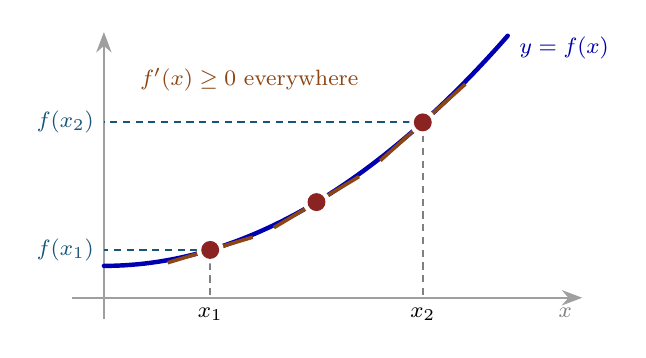
\begin{tikzpicture}[scale=1.35]
    % Axes
    \draw[axisln] (-0.3,0) -- (4.5,0) node[below left, gray]{\footnotesize $x$};
    \draw[axisln] (0,-0.2) -- (0,2.5);
    % Curve f(x) = 0.15 x^2 + 0.3
    \draw[curveln, blue!70!black, domain=0:3.8, samples=60]
      plot (\x, {0.15*\x*\x+0.3});
    \node[blue!70!black, right] at (3.82,2.35) {\footnotesize $y = f(x)$};
    % Tangent segments (slope f'(x) >= 0 everywhere)
    \draw[mAccent, line width=1.3pt] (0.6,0.33) -- (1.4,0.57);
    \draw[mAccent, line width=1.3pt] (1.6,0.66) -- (2.4,1.14);
    \draw[mAccent, line width=1.3pt] (2.6,1.29) -- (3.4,2.01);
    \node[mAccent, right] at (0.25,2.05) {\footnotesize $f'(x) \geq 0$ everywhere};
    % Two sample points: f(x_1) <= f(x_2)
    \draw[projln, gray] (1,0.45) -- (1,0) node[below, black]{\footnotesize $x_1$};
    \draw[projln, gray] (3,1.65) -- (3,0) node[below, black]{\footnotesize $x_2$};
    \draw[projln, defcolor] (1,0.45) -- (0,0.45)
      node[left]{\footnotesize $f(x_1)$};
    \draw[projln, defcolor] (3,1.65) -- (0,1.65)
      node[left]{\footnotesize $f(x_2)$};
    \dotpt{thmcolor}{(1,0.45)}
    \dotpt{thmcolor}{(2,0.9)}
    \dotpt{thmcolor}{(3,1.65)}
  \end{tikzpicture}
  \end{center}

  \note{
    In this picture, the blue curve has nonnegative slope at every point;
    the orange segments are tangent lines, and every one of them tilts
    upward or is flat. The claim of part "a" is that the curve as a whole
    can then never descend: pick any two marked points "x" sub 1 and "x"
    sub 2 with "x" sub 1 to the left, and as the dashed levels on the
    vertical axis show, the value of "f" at "x" sub 2 is at least the
    value at "x" sub 1. The mean value theorem is exactly the device that
    converts the pointwise slope condition into this two-point comparison.
    Here is the proof.
  }
\end{frame}

% --- Build 1/2 ---
\begin{frame}{Proof of Theorem 5.11}
  \begin{proofblock}{One equation proves all three parts}
    Fix $x_1 < x_2$ in $(a, b)$. Apply Theorem 5.10 to $[x_1, x_2]$:
    \[
      f(x_2) - f(x_1) = (x_2 - x_1)\, f'(x)
      \quad \text{for some } x \in (x_1, x_2).
    \]
  \end{proofblock}

  \note{
    The whole proof is one application of the mean value theorem. Take any
    two points "x" sub 1 less than "x" sub 2 inside the interval. On the
    closed interval between them, "f" is differentiable, hence continuous,
    so Theorem 5.10 applies: the difference of the function values equals
    the positive factor "x" sub 2 minus "x" sub 1, times the derivative at
    some intermediate point "x". Every conclusion can now be read off
    from this single equation.
  }
\end{frame}

% --- Build 2/2 ---
\begin{frame}{Proof of Theorem 5.11}
  \begin{proofblock}{One equation proves all three parts}
    Fix $x_1 < x_2$ in $(a, b)$. Apply Theorem 5.10 to $[x_1, x_2]$:
    \[
      f(x_2) - f(x_1) = (x_2 - x_1)\, f'(x)
      \quad \text{for some } x \in (x_1, x_2).
    \]
  \end{proofblock}

  \vspace{0.3em}
  \begin{hlbox}
  Since $x_2 - x_1 > 0$, the sign of $f(x_2) - f(x_1)$ is the sign of $f'(x)$:

  \begin{itemize}
    \item[(a)] $f' \geq 0$ on $(a,b)$ $\;\Longrightarrow\;$
      $f(x_2) \geq f(x_1)$: \alert{increasing}
    \item[(b)] $f' = 0$ on $(a,b)$ $\;\Longrightarrow\;$
      $f(x_2) = f(x_1)$: \alert{constant}
    \item[(c)] $f' \leq 0$ on $(a,b)$ $\;\Longrightarrow\;$
      $f(x_2) \leq f(x_1)$: \alert{decreasing} \hfill $\blacksquare$
  \end{itemize}
  \end{hlbox}

  \note{
    Now read off the three parts. The factor "x" sub 2 minus "x" sub 1 is
    positive, so the difference of function values has the same sign as
    the derivative at the intermediate point. If the derivative is
    nonnegative everywhere, the difference is nonnegative, so "f" is
    increasing; that is part "a". If the derivative vanishes everywhere,
    the difference is zero for every pair of points, so "f" is constant;
    part "b". If the derivative is nonpositive, "f" is decreasing; part
    "c". Since "x" sub 1 and "x" sub 2 were arbitrary, the proof is
    complete.
  }
\end{frame}
}

{
\usebackgroundtemplate{%
  
\includegraphics[width=\paperwidth,height=\paperheight,keepaspectratio=false]{chapter_05_bg_05.png}%
}
\section{Summary}

% --- Build 1/4 ---
\begin{frame}{Summary}
  \begin{hlbox}
  \textbf{Key takeaways from this section:}
  \begin{itemize}
    \item \alert{Theorem 5.8 (Fermat):} at an interior local extremum where
      $f'$ exists, $f'(x) = 0$
  \end{itemize}
  \end{hlbox}

  \note{
    Let's review what we covered. First, Theorem 5.8, Fermat's theorem: if
    a function defined on an interval has a local maximum or minimum at an
    interior point, and the derivative exists there, the derivative must
    be zero. The proof compared the signs of the one-sided difference
    quotients. This is the tool that locates candidates for extrema and
    powers the proofs that followed.
  }
\end{frame}

% --- Build 2/4 ---
\begin{frame}{Summary}
  \begin{hlbox}
  \textbf{Key takeaways from this section:}
  \begin{itemize}
    \item \alert{Theorem 5.8 (Fermat):} at an interior local extremum where
      $f'$ exists, $f'(x) = 0$
    \item \alert{Theorem 5.9 (Generalized MVT):}
      $[f(b)-f(a)]\,g'(x) = [g(b)-g(a)]\,f'(x)$, via an auxiliary function
  \end{itemize}
  \end{hlbox}

  \note{
    Second, the generalized mean value theorem. For two functions
    continuous on the closed interval and differentiable inside, the
    increments and derivatives balance at some interior point. The proof
    technique deserves its own mention: build an auxiliary function with
    equal endpoint values, then apply the extreme value theorem and
    Fermat's theorem. Auxiliary functions of this kind reappear
    throughout analysis.
  }
\end{frame}

% --- Build 3/4 ---
\begin{frame}{Summary}
  \begin{hlbox}
  \textbf{Key takeaways from this section:}
  \begin{itemize}
    \item \alert{Theorem 5.8 (Fermat):} at an interior local extremum where
      $f'$ exists, $f'(x) = 0$
    \item \alert{Theorem 5.9 (Generalized MVT):}
      $[f(b)-f(a)]\,g'(x) = [g(b)-g(a)]\,f'(x)$, via an auxiliary function
    \item \alert{Theorem 5.10 (MVT):} $f(b) - f(a) = (b-a)\,f'(x)$ ---
      the bridge from local to global
  \end{itemize}
  \end{hlbox}

  \note{
    Third, the mean value theorem itself, obtained from the generalized
    version by taking "g" to be the identity. Somewhere inside the
    interval, the instantaneous rate of change equals the average rate of
    change; geometrically, some tangent is parallel to the secant. This
    is the bridge between local information about the derivative and
    global information about the function, and it is arguably the most
    frequently used theorem of differential calculus.
  }
\end{frame}

% --- Build 4/4 ---
\begin{frame}{Summary}
  \vspace{-0.5em}
  \begin{hlbox}
  \textbf{Key takeaways from this section:}
  \begin{itemize}
    \item \alert{Theorem 5.8 (Fermat):} at an interior local extremum where
      $f'$ exists, $f'(x) = 0$
    \item \alert{Theorem 5.9 (Generalized MVT):}
      $[f(b)-f(a)]\,g'(x) = [g(b)-g(a)]\,f'(x)$, via an auxiliary function
    \item \alert{Theorem 5.10 (MVT):} $f(b) - f(a) = (b-a)\,f'(x)$ ---
      the bridge from local to global
    \item \alert{Theorem 5.11:} sign of $f'$ $\Rightarrow$ increasing / constant / decreasing
  \end{itemize}

  \vspace{-0.4em}
  \textbf{Coming up next:} \emph{The Continuity of Derivatives} ---
  derivatives satisfy the intermediate value property, even when discontinuous!
  \end{hlbox}

  \note{
    Finally, Theorem 5.11: the sign of the derivative controls
    monotonicity. Nonnegative derivative means increasing, identically
    zero means constant, nonpositive means decreasing, and all three
    conclusions fell out of one application of the mean value theorem. In
    the next episode we ask a subtle question: how badly can a derivative
    be discontinuous? We will prove a surprising result: every derivative,
    continuous or not, satisfies the intermediate value property, just
    like continuous functions do. See you there.
  }
\end{frame}
}

\end{document}
